\chapter{Presentation of results}
\section{Introduction}
This chapter presents a comprehensive overview of the system's results, including the user interface design, system functionalities, and the development environment used to build Elder Care Connect. The chapter is structured to provide a clear understanding of how the system operates through relevant screenshots, descriptions of core features, and an analysis of system performance. Additionally, this section discusses the tools, frameworks, and programming environments that were utilized during development, highlighting the technical aspects that contribute to the system’s efficiency and reliability.
\section{System Interfaces and User Experience}
The Elder Care Connect system has been designed with a user-centric approach, ensuring accessibility and ease of use for both elderly users and caregivers. The following subsections provide a detailed presentation of the user interfaces, highlighting key features with accompanying screenshots.
\begin{enumerate}
    \item \textbf{Login and Authentication System}
    \begin{itemize}
        \item A secure login system using google authentication and also email and password authentication with role-based access control (caregivers and elderly users).
    \end{itemize}
    \item \textbf{Dashboard Overview}
        \begin{itemize}
            \item The dashboard serves as the central hub, providing quick access to key functionalities.
            \item Features include an overview of medication schedules, chat notifications, and location tracking.
            \end{itemize}
    \item \textbf{Medication Reminder Management}
            \begin{itemize}
                \item A user-friendly interface allowing caregivers to set up medication schedules with time-based alerts.
                \item Elderly users receive visual reminders for medication intake.
            \end{itemize}
    \item \textbf{Real-Time Chat and Communication}
            \begin{itemize}
                \item Secure WebSocket-based real-time chat for seamless communication between caregivers and elderly users.
                \item Supports text, share reminders and location for enhanced interaction.
            \end{itemize}
    \item \textbf{Emergency Alerts}
                \begin{itemize}
                    \item Integrated emergency alert notifications.
                \end{itemize}             
\end{enumerate}
\section{Programming Environment and Technologies Used}
To develop the Elder Care Connect system, a modern technology stack was employed to ensure high performance, scalability, and security. The following tools and frameworks were integral to the development process:
\begin{enumerate}
    \item \textbf{Frontend Development}
        \begin{itemize}
            \item \textbf{Node.js:} Used for building a dynamic and responsive user interface with reusable components.
            \item \textbf{Tailwind CSS:} Applied for designing a visually appealing and accessible UI.
        \end{itemize}
    \item \textbf{Backend Development}
        \begin{itemize}
            \item \textbf{Node.js and Express.js:} Powering the backend API with RESTful services for seamless communication between the frontend and database.
            \item \textbf{WebSocket.io:} Used for real-time chat and live updates.
            \item \textbf{JWT (JSON Web Tokens):} Implemented for secure user authentication and authorization.
        \end{itemize}
    \item \textbf{Database Management}
    \begin{itemize}
        \item \textbf{MongoDB:} A NoSQL database used for storing user information, medication schedules, and chat history.
        \item \textbf{Firebase:} Utilized for real-time data synchronization, authentication, and cloud storage, ensuring seamless data access and backup \cite{firebase_docs}.
    \end{itemize}
    \item \textbf{Security and Data Protection}
        \begin{itemize}
            \item \textbf{Bcrypt.js:} Used for hashing user passwords to enhance security.
            \item \textbf {SSL Encryption:} Ensures secure data transmission over the network.
        \end{itemize}
\end{enumerate}
\section{Summary}
This chapter provided an in-depth overview of the Elder Care Connect system’s interfaces, functionalities, and technical implementation. Through the presentation of screenshots and descriptions, we demonstrated how the system facilitates seamless communication and care management for elderly individuals and caregivers. Furthermore, the programming environment and technology stack were detailed to highlight the system’s robust architecture and security measures. The performance evaluation results confirm the system’s reliability, scalability, and efficiency in real-world applications. These findings serve as a testament to the project’s success in addressing key challenges in elderly care and provide a foundation for future enhancements.
\newpage
%%%%%%% screenshots %%%%%%%%
\begin{figure}
    \centering
    \begin{minipage}{\textwidth}
        \centering
        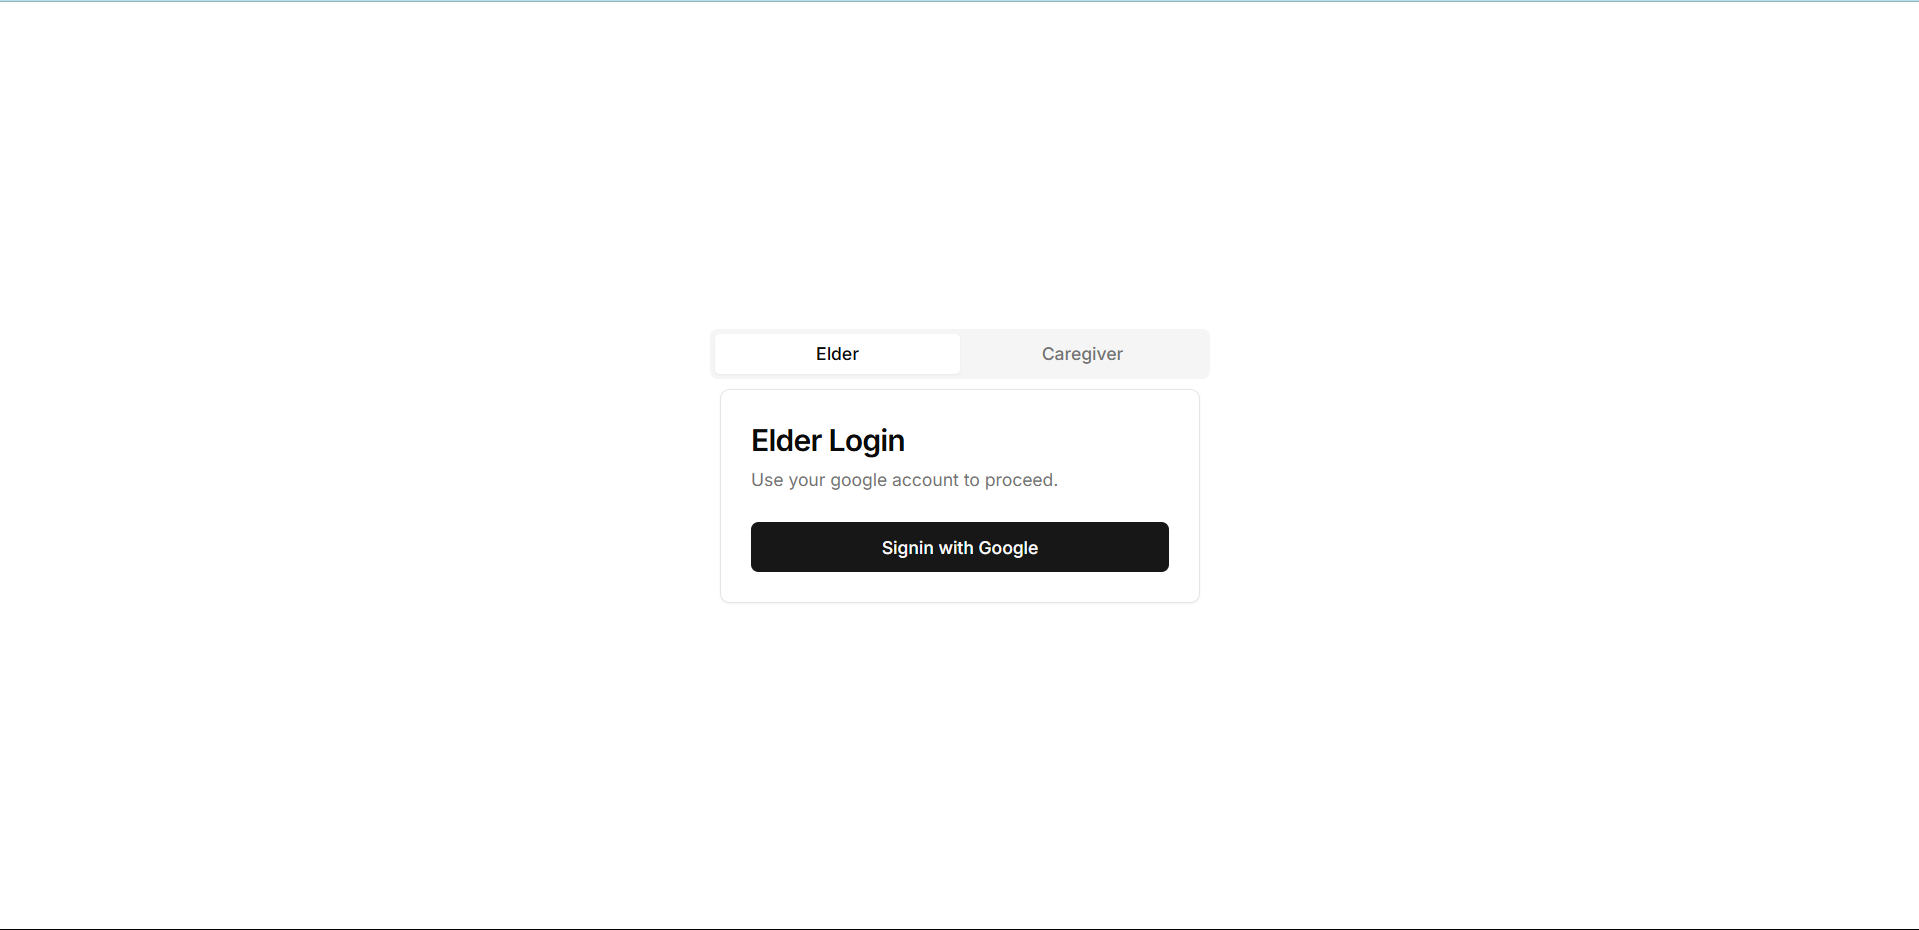
\includegraphics[width=0.9\textwidth]{login.png}
        \caption{Login Page}
        \label{fig:login}
    \end{minipage}
    \vspace{5pt}
    \begin{minipage}{\textwidth}
        \centering
        \includegraphics[width=0.9\textwidth]{dashboard.png}
        \caption{Elderly User Dashboard}
        \label{fig:elderly_dashboard}
    \end{minipage}
    \vspace{5pt}
    \begin{minipage}{\textwidth}
        \centering
       \includegraphics[width=0.9\textwidth]{dashboard.png}
        \caption{Caregiver Dashboard}
        \label{fig:caregiver_dashboard}
    \end{minipage}
    \vspace{5pt}
\end{figure}

\begin{figure}
    \centering
    \begin{minipage}{\textwidth}
        \centering
        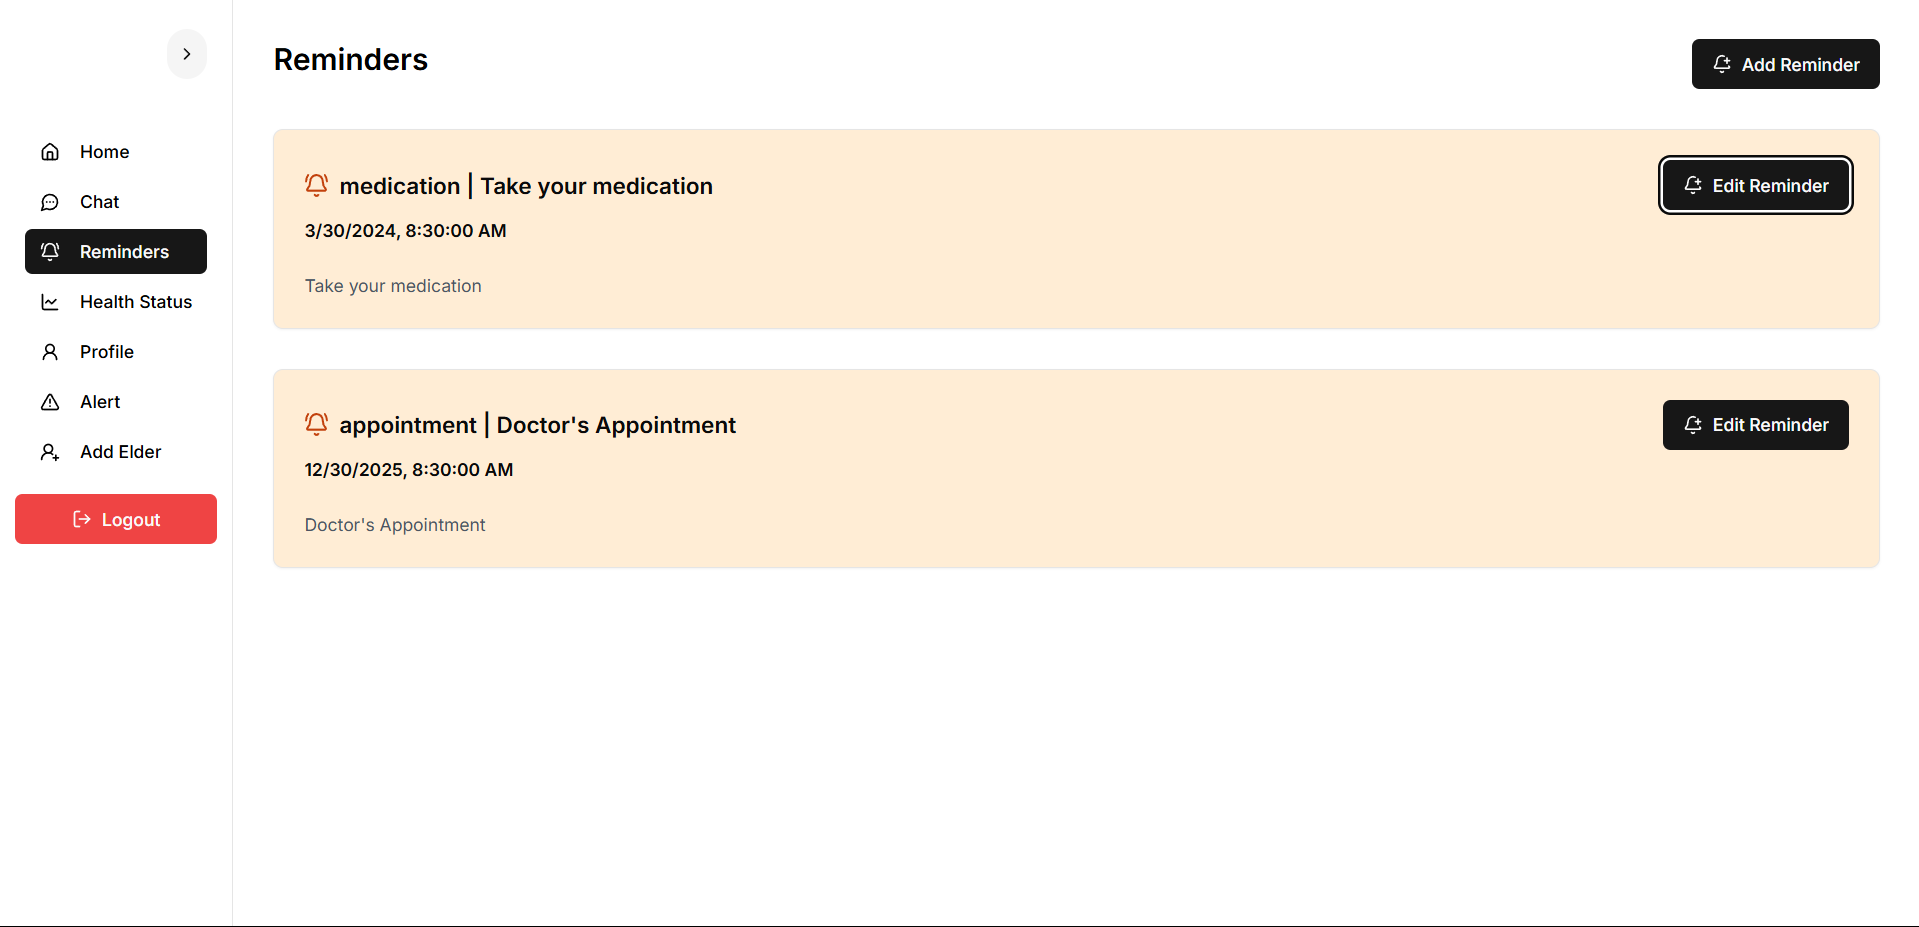
\includegraphics[width=0.9\textwidth]{reminders.png}
        \caption{Reminders\\}
        \label{fig:reminders}
    \end{minipage}
    \vspace{5pt}
    \begin{minipage}{\textwidth}
        \centering
        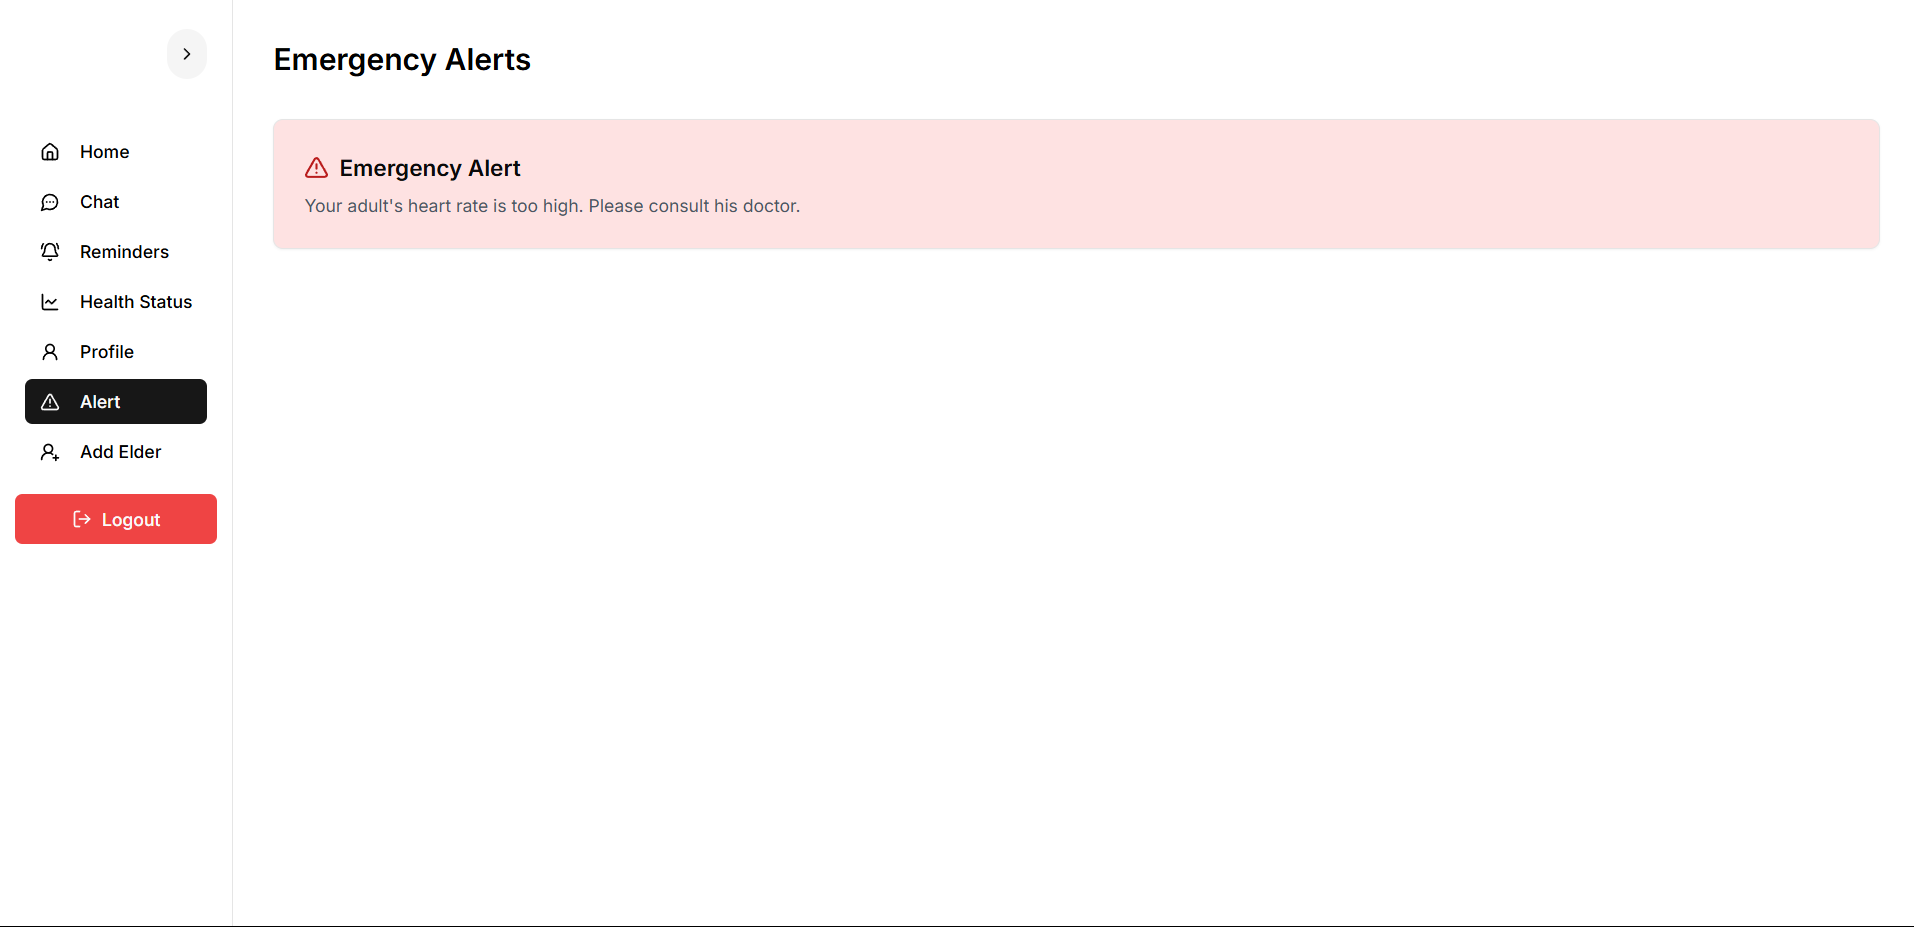
\includegraphics[width=0.9\textwidth]{alert.png}
        \caption{Alerts}
        \label{fig:alerts}
    \end{minipage}
    \vspace{5pt}
    \begin{minipage}{\textwidth}
        \centering
        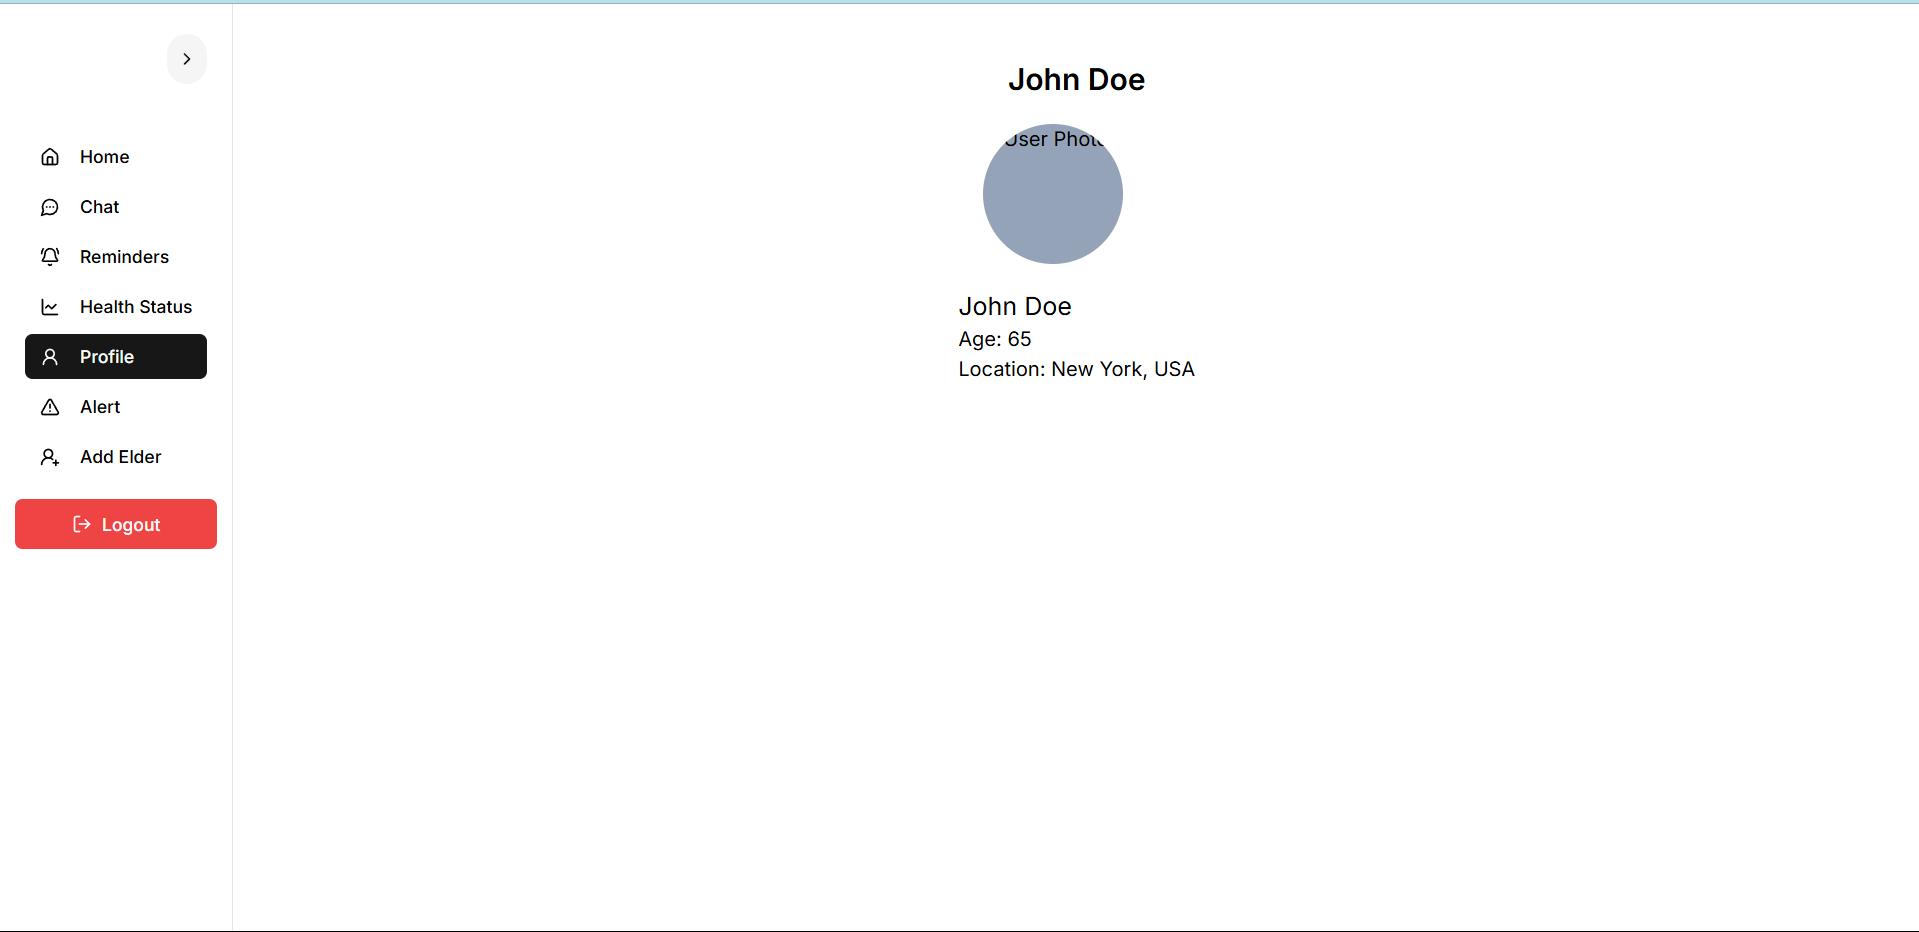
\includegraphics[width=0.9\textwidth]{profile.png}
        \caption{Profile}
        \label{fig:profile}
    \end{minipage}
    \vspace{5pt}
\end{figure}

\begin{figure}
    \centering
    \begin{minipage}{\textwidth}
        \centering
        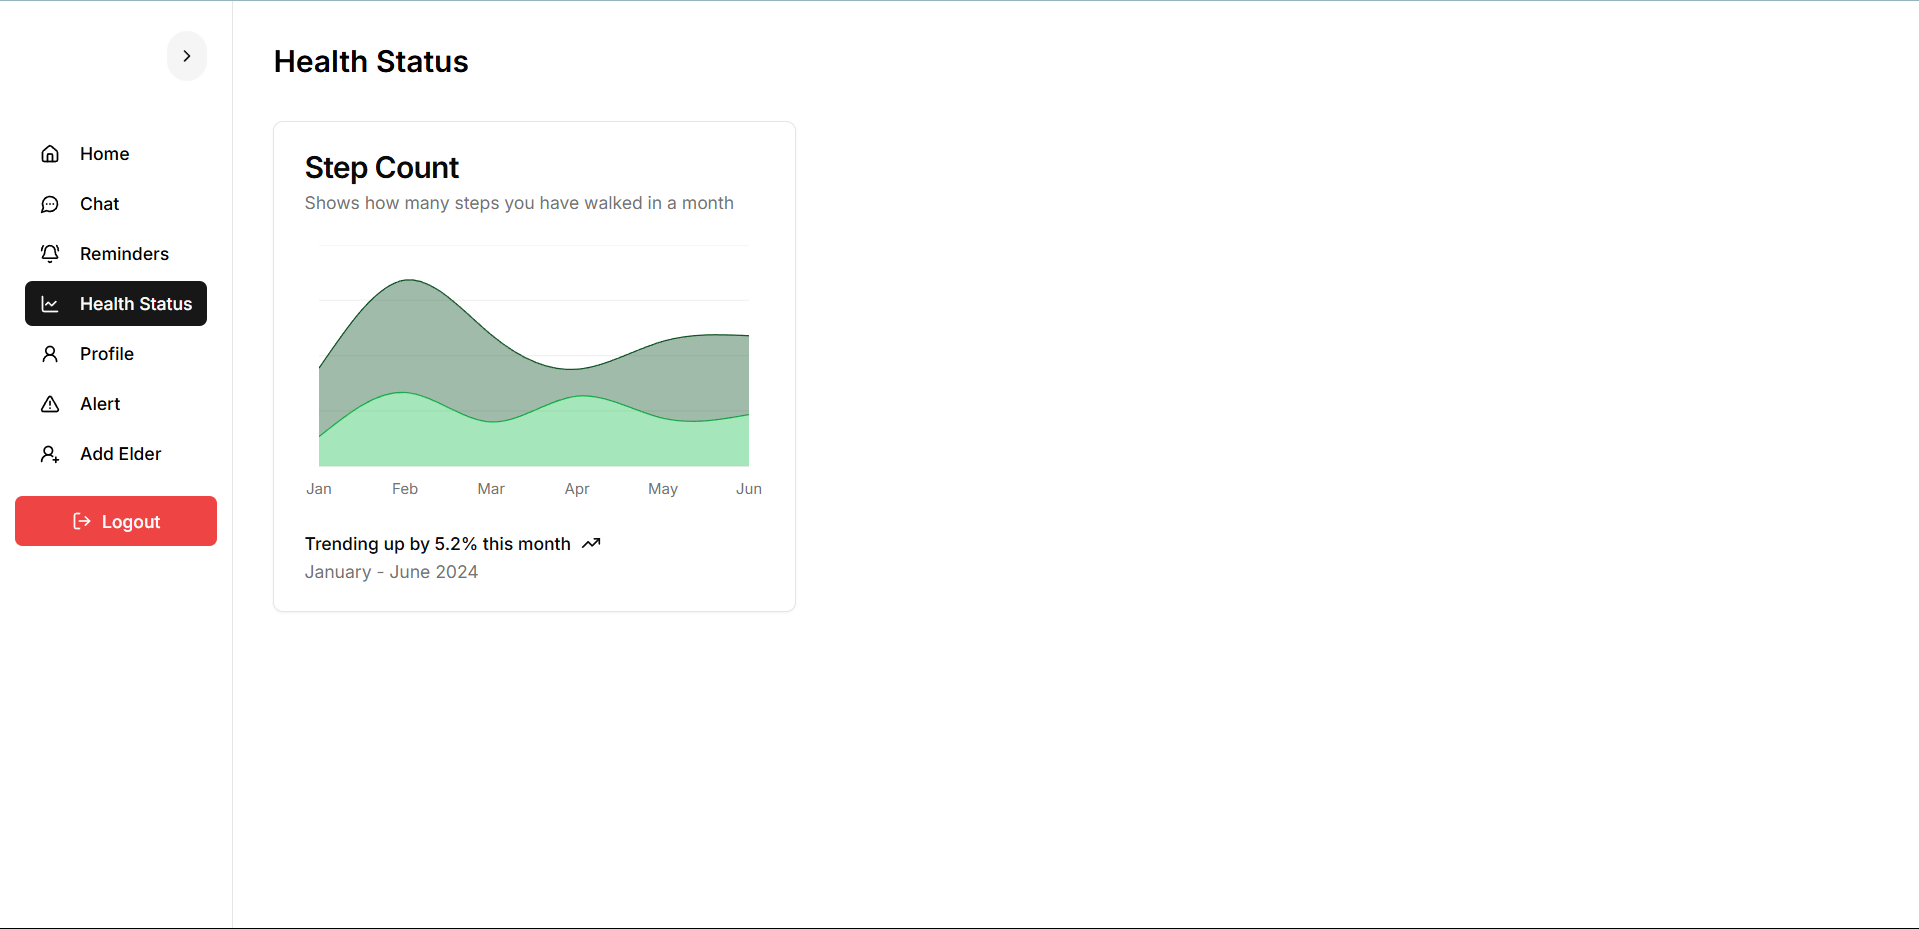
\includegraphics[width=0.9\textwidth]{health data.png}
        \caption{Health Status}
        \label{fig:health_status}
    \end{minipage}
    \vspace{5pt}
    \begin{minipage}{\textwidth}
        \centering
        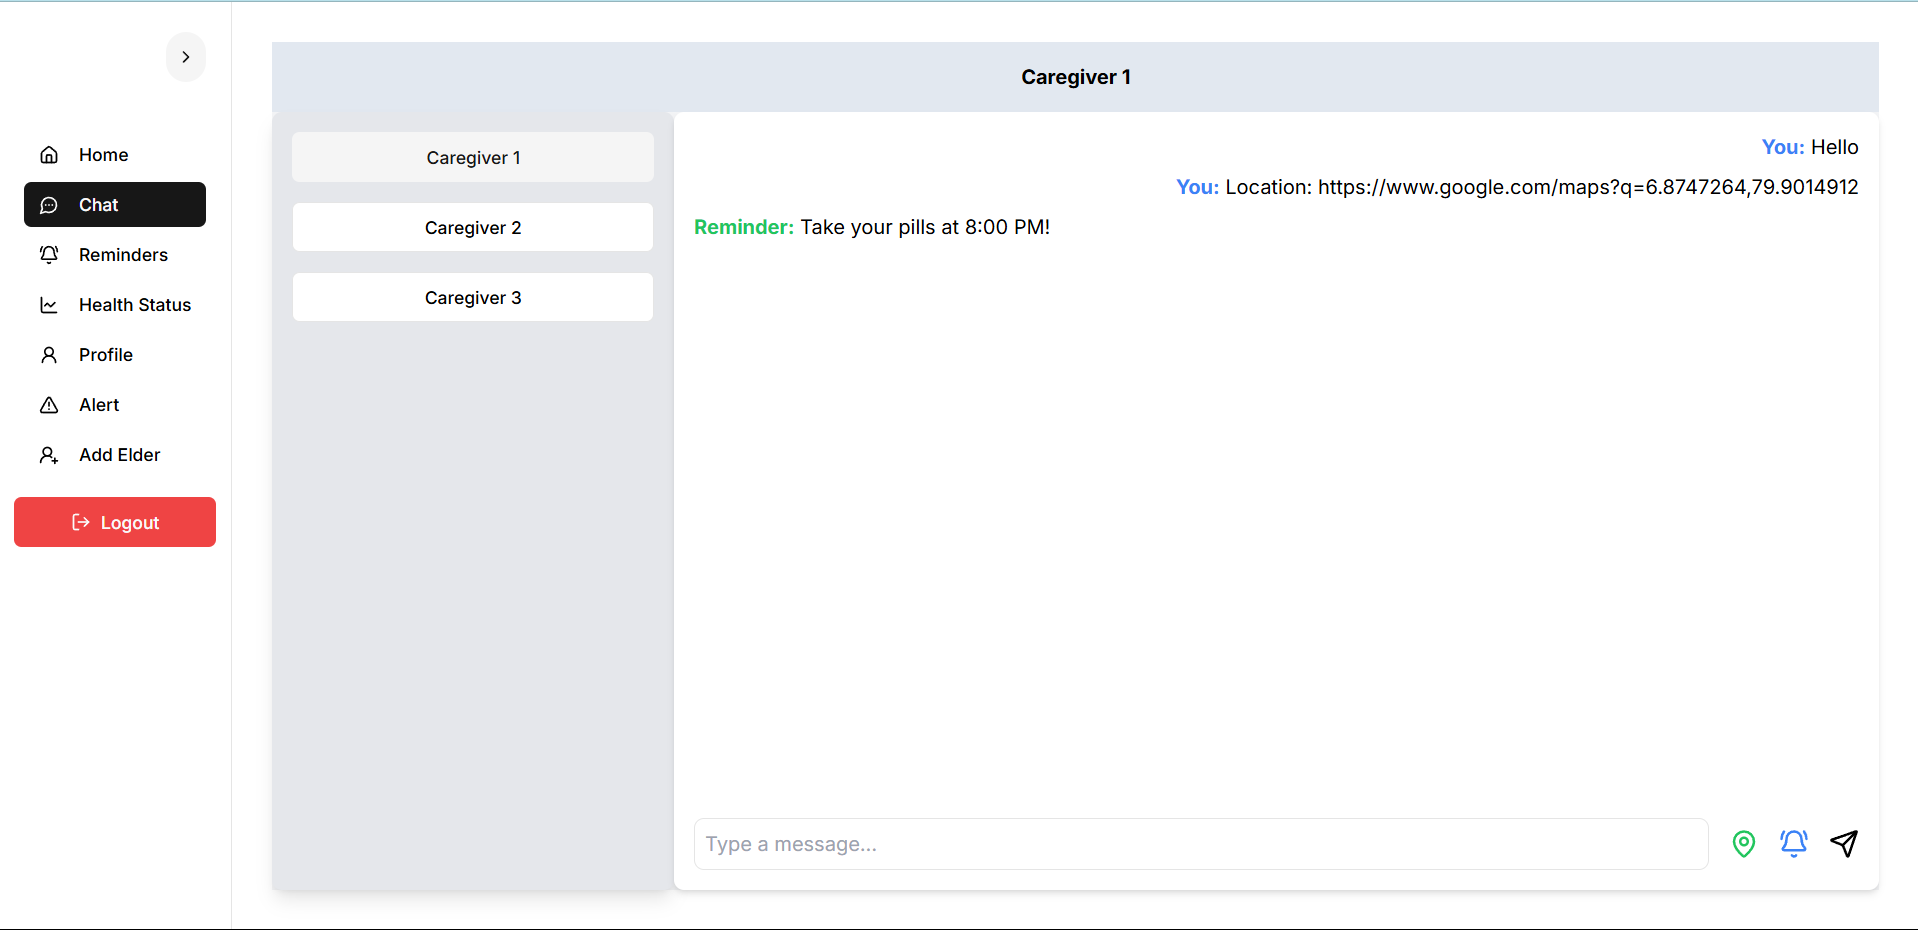
\includegraphics[width=0.9\textwidth]{chat.png}
        \caption{Chat}
        \label{fig:chat}
    \end{minipage}
    \vspace{5pt}
    \begin{minipage}{\textwidth}
        \centering
        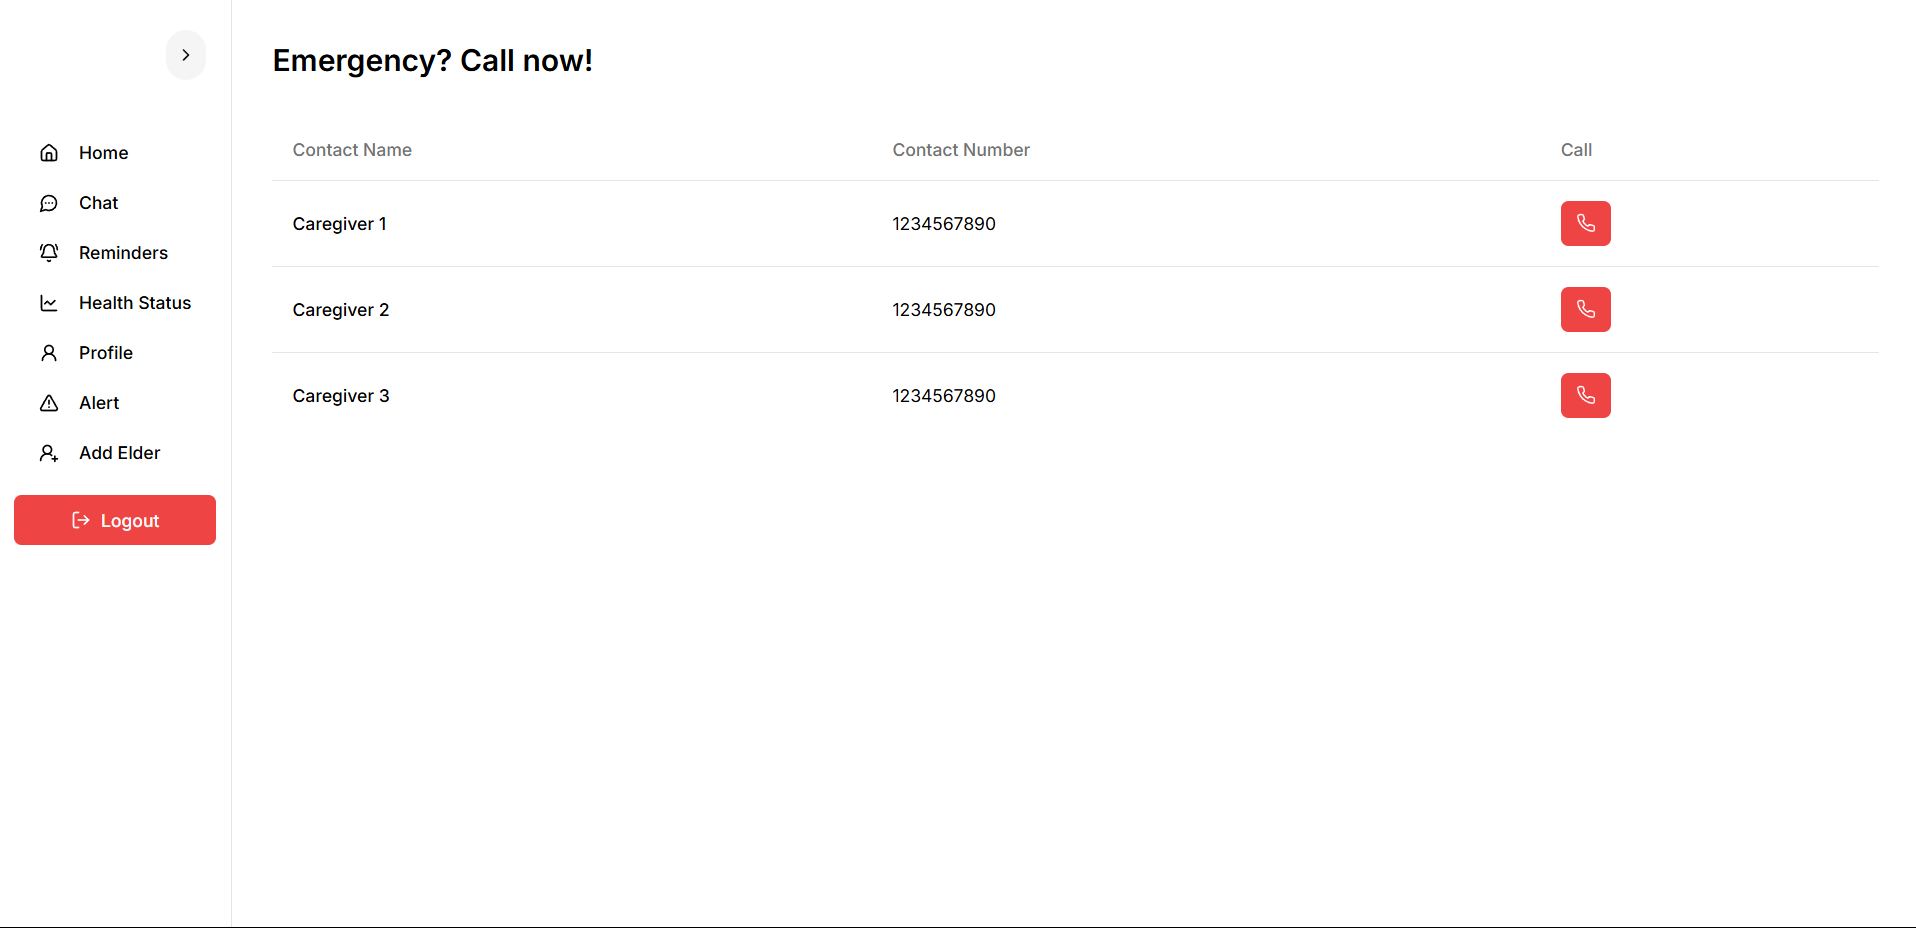
\includegraphics[width=0.9\textwidth]{emergency contact.png}
        \caption{Emergency Call}
        \label{fig:emergency_call}
    \end{minipage}
    \vspace{5pt}
\end{figure}